\subsection{Decoding Voltmeter Sensitivity: Why Ohms per Volt Matter!}

\begin{tcolorbox}[colback=gray!10, colframe=black, title=E4B02`]
What is the significance of voltmeter sensitivity expressed in ohms per volt? 
\begin{enumerate}[label=\Alph*.]
    \item \textbf{The full scale reading of the voltmeter multiplied by its ohms per volt rating is the input impedance of the voltmeter}
    \item The reading in volts multiplied by the ohms per volt rating will determine the power drawn by the device under test
    \item The reading in ohms divided by the ohms per volt rating will determine the voltage applied to the circuit
    \item The full scale reading in amps divided by ohms per volt rating will determine the size of shunt needed
\end{enumerate} \end{tcolorbox}

\subsubsection{Related Concepts}

The sensitivity of a voltmeter is a crucial characteristic that provides insight into how the voltmeter will affect the circuit being measured. Specifically, the sensitivity expressed in ohms per volt quantifies the input impedance of the voltmeter. This is important because a voltmeter with a higher sensitivity (higher ohms per volt rating) will draw less current from the circuit it is measuring, thus minimizing the influence on the measured voltage.

To elaborate further, for a voltmeter, sensitivity indicates that for each volt of reading on the meter, it has a certain impedance in ohms. For example, if a voltmeter has a sensitivity of 1,000 ohms/volt and is used to take a reading of 5 volts, its input impedance can be calculated as follows:

\[
Z_{in} = \text{Sensitivity} \times \text{Voltmeter Reading} = 1000 \, \Omega/\text{V} \times 5 \, \text{V} = 5000 \, \Omega
\]

This calculation indicates that while measuring 5 volts, the voltmeter presents a load of 5000 ohms to the circuit.

The correct answer to the question is option A, which highlights that the full-scale reading of the voltmeter multiplied by its ohms per volt rating gives the input impedance.

\subsubsection{Importance of Input Impedance}

The input impedance of a voltmeter needs to be significantly higher than the impedance of the circuit being measured. If the voltmeter's input impedance is low, it will draw a considerable amount of current, which will alter the characteristics of the circuit and lead to inaccurate voltage readings. Ideally, the voltmeter should not load the circuit under test.

\begin{center}
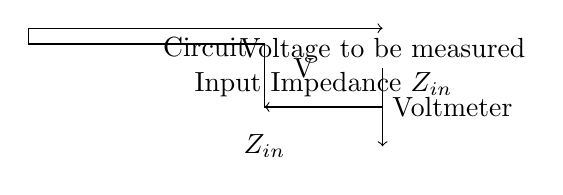
\begin{tikzpicture}
    \draw[->] (0,0) -- (4.5,0) node[midway, below] {Circuit} node[below] {Voltage to be measured};
    \draw[->] (4.5,-0.5) -- (4.5,-1.5) node[midway, right] {Voltmeter};
    \draw[->] (4.5,-1) -- (3,-1) node[midway, above] {Input Impedance $Z_{in}$};

    \draw (3,-1) -- (3,-0.2) -- (0,-0.2) -- (0,0);
    \draw[dashed] (3,-1) -- (4.5,-1);
    \node at (3.5, -0.5) {V};
    \node at (3, -1.5) {$Z_{in}$};
\end{tikzpicture}
\end{center}

In conclusion, understanding voltmeter sensitivity and its representation in ohms per volt is fundamental for proper voltage measurement in electronic circuits. Choosing a voltmeter with the right specifications and understanding the implications of its sensitivity can greatly improve measurement accuracy and reliability. 
